%narms.tex, an example driver file for Balkema documents.

%use the following for A4 paper:
\documentclass[12pt,a4paper,twocolumn,fleqn]{narms}


% packages needed
%\usepackage{subfigure}
\usepackage{epsfig}
\usepackage{timesmt}
\mathindent=0pt%

\usepackage{chicaco}

% custom packages
\usepackage{amsmath}
\usepackage[noabbrev]{cleveref}
\usepackage{dsfont}
\setlength{\mathindent}{0cm}
%\usepackage{subfig}
\usepackage{graphicx}
\usepackage{subcaption}
\usepackage{siunitx}
\usepackage[font=small,justification=justified,singlelinecheck=false]{caption}


% setting math equation indent from left 0pts

\mathindent=0pt%

% use this for chicaco style reference
% Author references
% IMPORTANT: Author wants to format references in chicaco style Author must use BiBTex
% IMPORTANT: Author wants to format numbered references remove chicaco style file and \bibliographystyle{chicaco}

\usepackage{chicaco}

%  \cite{key}
%    which produces citations with full author list and year.
%    eg. (Brown 1978; Jarke, Turner, Stohl, et al. 1985)

%  \citeNP{key}
%    which produces citations with full author list and year, but without
%    enclosing parentheses:
%    eg. Brown 1978; Jarke, Turner & Stohl 1985

%  \citeA{key}
%    which produces citations with only the full author list.
%    eg. (Brown; Jarke, Turner & Stohl)

%  \citeANP{key}
%    which produces citations with only the full author list, without
%    parentheses eg. Brown; Jarke, Turner & Stohl

%  \citeN{key}
%    which produces citations with the full author list and year, but
%    can be used as nouns in a sentence; no parentheses appear around
%    the author names, but only around the year.
%      eg. Shneiderman (1978) states that......
%    \citeN should only be used for a single citation.

%  \shortcite{key}
%    which produces citations with abbreviated author list and year.

%  \shortciteNP{key}
%    which produces citations with abbreviated author list and year.

%  \shortciteA{key}
%    which produces only the abbreviated author list.

%  \shortciteANP{key}
%    which produces only the abbreviated author list.

%  \shortciteN{key}
%    which produces the abbreviated author list and year, with only the
%    year in parentheses. Use with only one citation.

%  \citeyear{key}
%    which produces the year information only, within parentheses.

%  \citeyearNP{key}
%    which produces the year information only.


%%%%%%%%%%%%%%%%%%%%%%%%%%%%%%%%%%%%%%%%%%%%%%%%%%%%%%%%%%%%%%%%%%%
%%%  All this stuff is from modifying the article.cls for Balkema
%%%  specifications.

%\title{...}
%\author{...}
%use \aff for author affiliations
% use \authornext for from second author
% empty line space between multiple authors
%\abstract{...}
%\maketitle{}

%%%%%%% Style for TABLES
% insert tabular command inside \tabletext{} this will produce tables in 10pts


\begin{document}
\title{Effect of initial volume fraction on the collapse of granular columns in fluid}
\author{{K. Kumar} \\
{\aff{Computational Geomechanics Research Group, Department of Engineering, University of Cambridge, UK}} \\
\\
{\authornext{J-Y. Delenne}}\\
{\aff{IATE, UMR 1208 INRA-CIRAD-Montpellier Supagro-UM2, University of Montpellier 2, France.}} \\
\\
{\authornext{K. Soga}}\\
{\aff{Department of Civil and Environmental Engineering, University of California, Berkeley, USA.}}}

\date{}% No date.

\abstract{This paper investigates the effect of initial volume fraction on the runout characteristics of granular column collapse in a fluid. Two-dimensional sub-grain scale numerical simulations are performed to understand the flow dynamics of granular collapse in a fluid. The Discrete Element (DEM) technique is coupled with the Lattice Boltzmann Method (LBM), for fluid-grain interactions, to understand the evolution of submerged granular flows. The fluid phase is simulated using Multiple-Relaxation-Time LBM (LBM-MRT) for numerical stability. In order to simulate interconnected pore space in 2D, a reduction in the radius of the grains (hydrodynamic radius) is assumed during LBM computations. A parametric analysis is performed to assess the influence of the granular characteristics (initial packing) on the evolution of flow and run-out distances. The volume of the initial packing is changed to simulate different stress conditions while maintaining the same aspect ratio. The influence of the stress condition on the run-out behaviour is studied for different permeabilities. The granular flow dynamics is investigated by analysing the effect of hydroplaning, water entrainment and viscous drag on the granular mass. The mechanism of energy dissipation, the shape of the flow front, water entrainment and evolution of packing density is used to explain the difference in the flow characteristics of loose and dense granular column collapse in a fluid.}

\maketitle

\section{INTRODUCTION}


The flow of dense granular material is a common phenomenon in engineering predictions, such as avalanches, landslides, and debris-flow modelling. Despite the huge amount of research that has gone into describing the behaviour of granular flows, a constitutive equation that describes the overall behaviour of a flowing granular material is still lacking. The initiation and propagation of submarine granular flows depend mainly on the slope, density, and quantity of the material destabilised. Although certain macroscopic models are able to capture the simple mechanical behaviours, the complex physical mechanisms that occur at the grain scale, such as the hydrodynamic instabilities, the formation of clusters, collapse, and transport, have largely been ignored~\shortcite{Topin2011}. The momentum transfer between the discrete and the continuous phases significantly affects the dynamics of the flow~\shortcite{Peker2007}. Grain-scale description of the granular material enriches the macro-scale variables,  which poorly account for the local rheology of the materials.  In order to describe the mechanism of saturated and/or immersed granular flows, it is important to consider both the dynamics of the solid phase and the role of the ambient fluid~\shortcite{Denlinger2001}. In particular, when the solid phase reaches a high volume fraction, it is important to consider the strong heterogeneity arising from the contact forces between the grains, the drag interactions which counteract the movement of the grains, and the hydrodynamic forces that reduce the weight of the solids inducing a transition from dense compacted to a dense suspended flow~\shortcite{Meruane2010}. The case of the collapse in presence of an interstitial fluid has been less studied. In this paper, we study the effect of permeability and initial density on the run-out evolution.

\section{LBM FORMULATION}

The Lattice Boltzmann Method is a `micro-particle' based numerical time-stepping procedure for the solution of incompressible fluid flows. Consider a 2D incompressible fluid flow with density $\rho$ and kinematic viscosity \textit{v}, in a rectangular domain \textit{\textbf{D}}. The fluid domain is divided into a rectangular grid or lattice, with the same spacing \textit{`h'} in both the \textit{x-} and the \textit{y-}directions. The present study focuses on two-dimensional problems, hence the \textit{D2Q9} momentum discretisation is adopted (see \shortciteN{He1997} for naming convention). The Multiple Relaxation Time LBM (LBM-MRT) is adopted in the present study for numerical stability. Further details about the modelling can be found in~\shortciteN{Kumar2015,Kumar2017}.

%**************************************************************************

\section{COUPLED LB - DEM FOR FLUID-PARTICLE INTERACTIONS}
The Lattice Boltzmann approach has the advantage of accommodating large particle sizes and the interaction between the fluid and the moving particles can be modelled through relatively simple fluid - particle interface treatments. Further, employing the Discrete Element Method (DE) to account for the particle/particle interaction naturally leads to a combined LB - DEM solution procedure. The Eulerian nature of the Lattice Boltzmann formulation, together with the common explicit time step scheme of both the Lattice Boltzmann and the Discrete Element makes this coupling strategy an efficient numerical procedure for the simulation of particle-fluid systems~\shortcite{Cook2004}. In order to capture the actual physical behaviour of the fluid-particle system, the boundary condition between the fluid and the particle is modelled as a non-slip boundary condition, i.e. the fluid near the particle should have similar velocity as the particle boundary. The solid particles inside the fluid are represented by lattice nodes. The discrete nature of lattice will result in stepwise representation of the surfaces. Very small lattice spacing is adopted to obtain smoother boundaries. 

\section{UNDERWATER GRANULAR FLOWS}
In this study, a 2D poly-disperse system ($d_{max}/d_{min} = 1.8$) of circular
discs in fluid was used to understand the behaviour of granular flows on
inclined planes (see~\Cref{fig:setup}). The soil column was modelled using
1000 discs of density \SI{2650}{\kg\per\cubic\meter} and a contact friction
angle of \SI{26}{\degree}. The collapse of the column was simulated inside a
fluid with a density of \SI{1000}{\kg\per\cubic\meter}  and a kinematic
viscosity of \SI{1e-6}{\square\meter\per\second}. The choice of a 2D geometry
has the advantage of cheaper computational effort than a 3D case, making it
feasible to simulate very large systems. A granular column of aspect ratio
`a' of 0.8 was used. Dry analyses were also performed to understand the effect
of hydrodynamic forces on the run-out distance in submerged granular flows.

\begin{figure}[htpb]
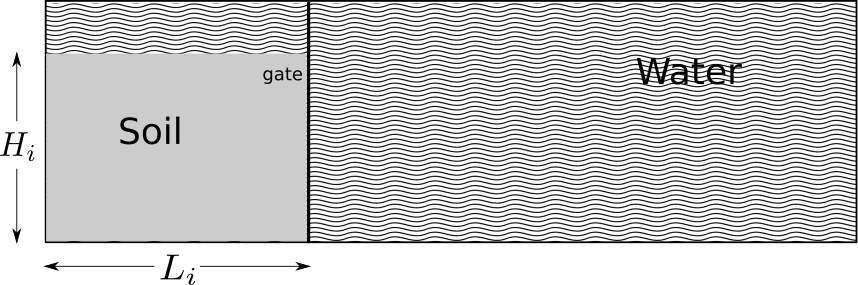
\includegraphics[width=0.97\columnwidth]{figs/geometry.png}
\caption{Underwater granular collapse set-up}
\label{fig:setup}
\end{figure}

\subsection{Effect of initial packing density}

\shortciteN{Rondon2011} observed that the loose packings flow rapidly on a time
scale proportional to the initial height and results in longer run-out distance 
in comparison to the dense packing. Hydroplaning occurs above a critical 
Froude's number of 0.4. The Froude's number is inversely related to the 
thickness of the flow and its density. Hence, for the same thickness of flow, a 
loose granular column will experience more hydroplaning than a dense granular 
flow. This effect might result in longer run-out behaviour in fluid than the 
dry condition for the same initial aspect ratio. The initial packing density 
and the permeability of a 2D granular column, with an aspect ratio of 0.8, are 
varied to understand their influence on the run-out behaviour. The run-out 
behaviour of the dense case (83\% packing density), is compared with a loose
granular column (79\% packing fraction). The permeability is varied by changing
the hydrodynamic radius from 0.7 \textit{R} (high permeability) to 0.95 \textit{R}
(low permeability). A hydrodynamic radius refers to the reduced grain diameter
used only in the LBM computation to simulate a 3D flow through a 2D system of rods.
See~\shortciteN{Kumar2015} for further details on the hydrodynamic radius.

\subsection{Dense granular collapse}
The normalised run-out for different hydrodynamic radii for a granular column 
with an initial aspect ratio of 0.8 for dense initial packing are presented 
in~\cref{fig:Runout_a08_dense}. The run-out increases with decrease in the 
permeability, which is equivalent to an increase in the hydrodynamic radius. 
An increase in the hydrodynamic radius from 0.7 to 0.95 \textit{R} increases 
the normalised run-out by 25\%. However, even under a very low permeability 
condition (\textit{r} = 0.95 \textit{R}), the run-out observed in fluid is 
shorter than the dry and the buoyant conditions. 

\begin{figure}[htpb]
\centering
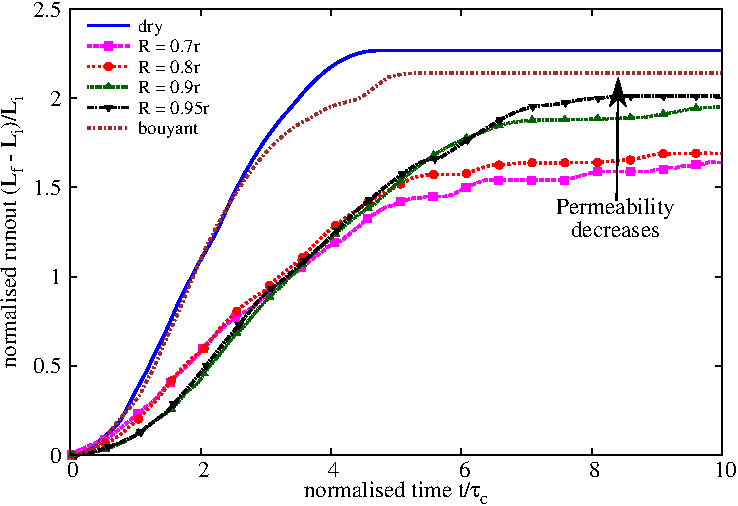
\includegraphics[width=0.9\linewidth]{figs/Runout_a08_dense}
\caption{Effect of permeability on the evolution of run-out for a column 
collapse in fluid (a = 0.8).}
\label{fig:Runout_a08_dense}
\end{figure}

At a high permeability (\textit{r} = 0.7 \textit{R}), the evolution of run-out 
at the initial stage is quicker, which means that the negative pore-pressure 
that is developed during the shearing along the shear-failure surface is 
dissipated faster. Even though the negative pore-pressure is dissipated, due to 
the development of negative pore-pressure the evolution of run-out in fluid is 
slower than its dry counterpart. The rate of pore-pressure dissipation 
decreases with decrease in the permeability. This can be observed by a flatter 
slope in the run-out evolution with decrease in the 
permeability.~\Cref{fig:PWP_ini_dense} shows the distribution of pore-pressure 
in high and low permeability granular media along the horizontal direction at a 
height of $10 \times d$ from the base. In LBM, the pore-pressure in fluid is a 
function of fluid density distribution functions. At time $t = \tau_c$, defined
as the critical time for the flow to be fully mobilised, the 
highly permeable (\textit{r} = 0.7 \textit{R}) granular column 
shows smaller negative pore-pressure in comparison to large negative 
pore-pressures observed in the shearing zone of a low permeable column 
(\textit{r} = 0.9 \textit{R}). This shows that not only does it take longer for the 
pore-pressure to dissipate with a decrease in permeability, but also results in 
almost twice the negative pore-pressure than what is observed in the high 
permeable case (\cref{fig:r095_PWP_ini_dense}). A 
high value of positive pore-pressure is observed at the face of the column 
in the low permeable condition. This indicates that the low permeable column 
fails as a continuous block undergoing a shear failure, which generates a very 
large negative pore-pressure along the failure surface. However, in the case of 
the high permeable column the failure is more localised with multiple negative 
pore-pressure spikes (\cref{fig:r07_PWP_ini_dense}).

\begin{figure}
\centering
\begin{subfigure}[t]{0.975\linewidth}
	\centering
    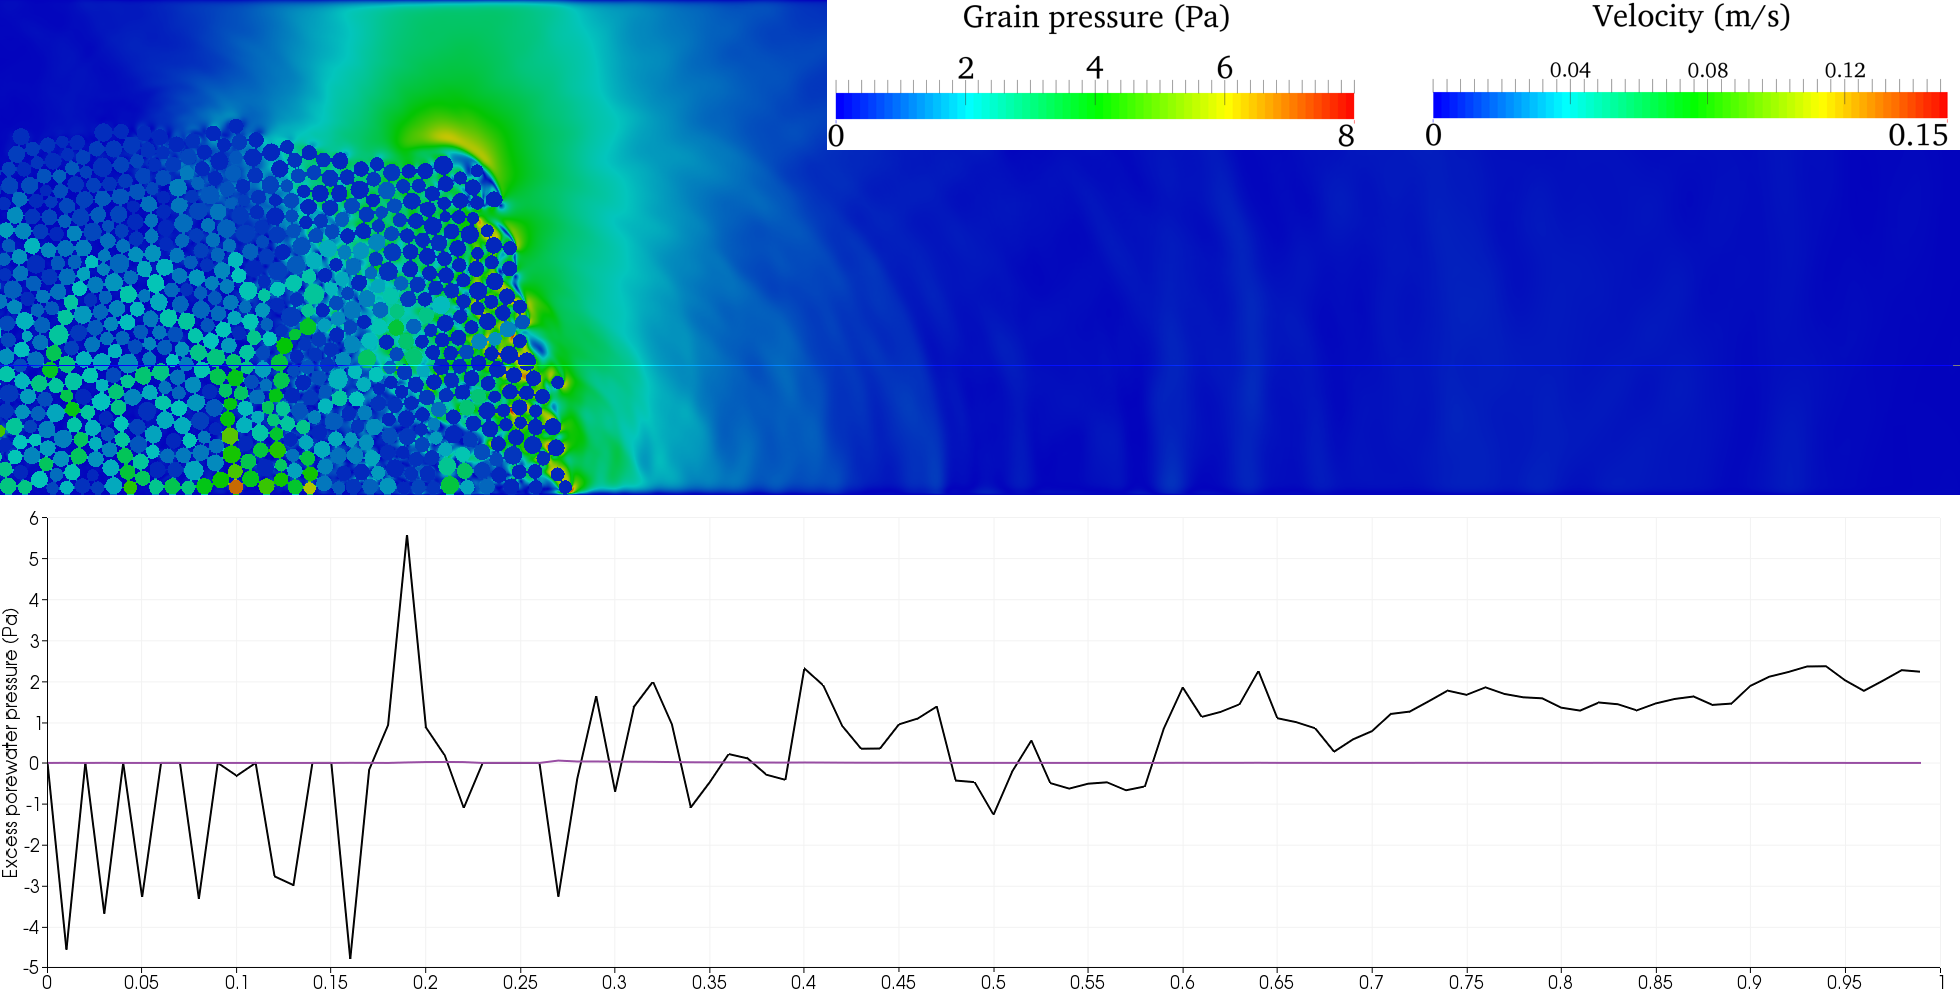
\includegraphics[width=\linewidth]{figs/a08/r07_PWP_ini_dense}
    \caption{High permeability (\textit{r} = 0.7 \textit{R}) - Pressure at the 
        bottom of the granular flow.}
    \label{fig:r07_PWP_ini_dense}
\end{subfigure} \\
\begin{subfigure}[t]{0.975\linewidth}
	\centering
    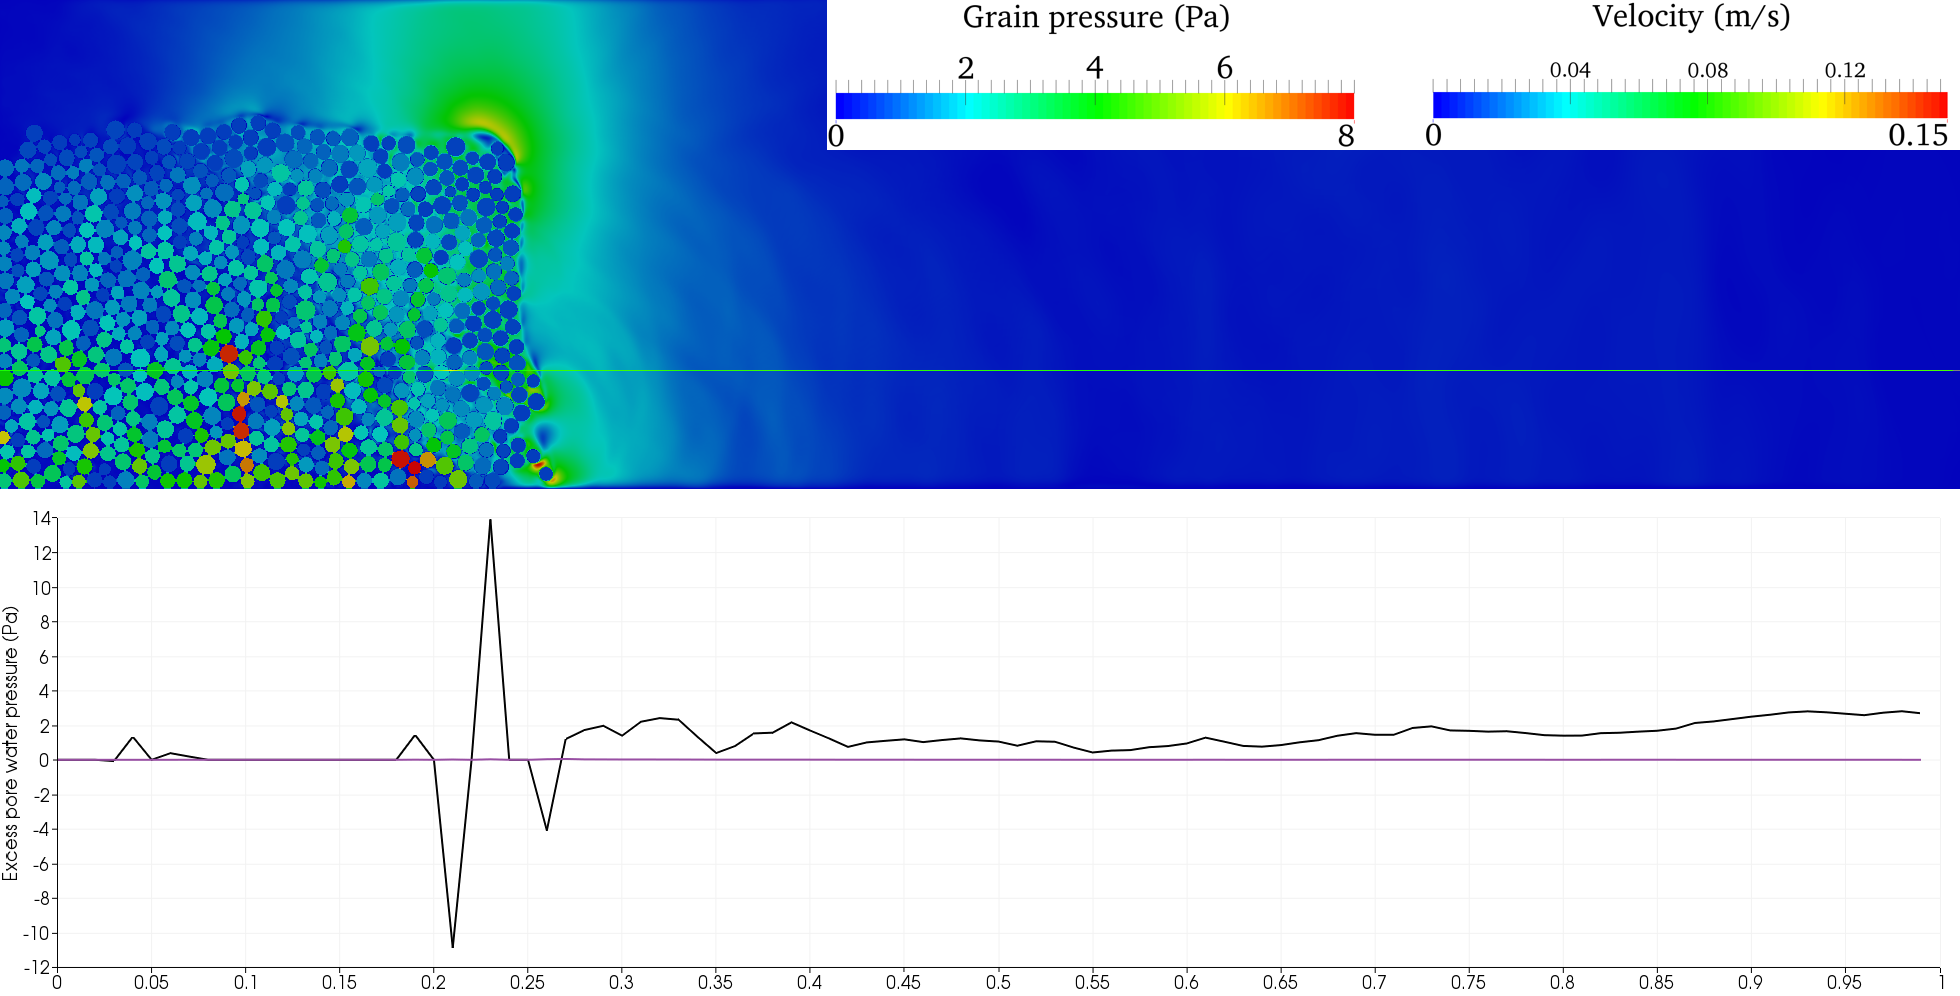
\includegraphics[width=\linewidth]{figs/a08/r095_PWP_ini_dense}
    \caption{Low permeability (\textit{r} = 0.95 \textit{R}) - Pressure at the 
        bottom of the granular flow.}
    \label{fig:r095_PWP_ini_dense}
\end{subfigure}
\caption{Effect of permeability on the excess pore water pressure distribution 
for a granular column collapse in fluid (a = 0.8 \& dense packing) at $t = 
\tau_c$ along the horizontal direction at a height of 10d from the base.}
\label{fig:PWP_ini_dense}
\end{figure}

Normalised kinetic energy evolution with time (\cref{fig:KExy_a08_dense}) shows that the 
low permeability column has a wider peak kinetic energy distribution in 
comparison to a sharp peak observed in the high permeability condition. This 
indicates the influence of lubrication, i.e., hydroplaning of the granular flow 
in low permeability conditions. The evolution of the horizontal kinetic energy 
with time reveals that the peak kinetic energy is sustained longer as the 
permeability of the granular material decreases . 
Although the peak kinetic energy is smaller in the low permeability case, the 
hydroplaning of the flowing granular mass results in a longer run-out 
distance.~\Cref{fig:r095_PWP_flow_dense} shows the 
distribution of pore-pressure for a dense granular column collapse in fluid 
along the bottom plane. A high positive pore-pressure is observed 
at the base of the granular flow at the flow front in low permeability 
condition indicating the occurrence of hydroplaning. The positive pore-pressure 
at the flow front decreases the effective stress thus the creating lubrication 
effect. The evolution of local packing density with time shows that the packing 
density decreases with decrease in permeability 
(\cref{fig:Packing_Density_a08_dense}). This drop 
in the value of packing density between $t = 2\tau_c$ and $t=3\tau_c$ 
corroborates with the duration of hydroplaning during which a large amount of 
water in entrained at the flow front.


\begin{figure}
    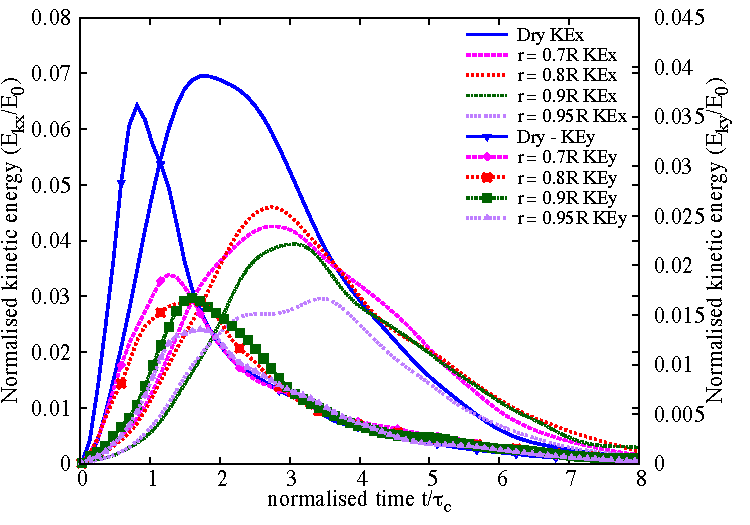
\includegraphics[width=\linewidth]{figs/KExy_a08_dense}
    \caption{Effect of permeability on the evolution of kinetic energies with time 
for a granular column collapse in fluid (a = 0.8).}
    \label{fig:KExy_a08_dense}
\end{figure}

\begin{figure}
\centering
\begin{subfigure}[t]{0.975\linewidth}
	\centering
    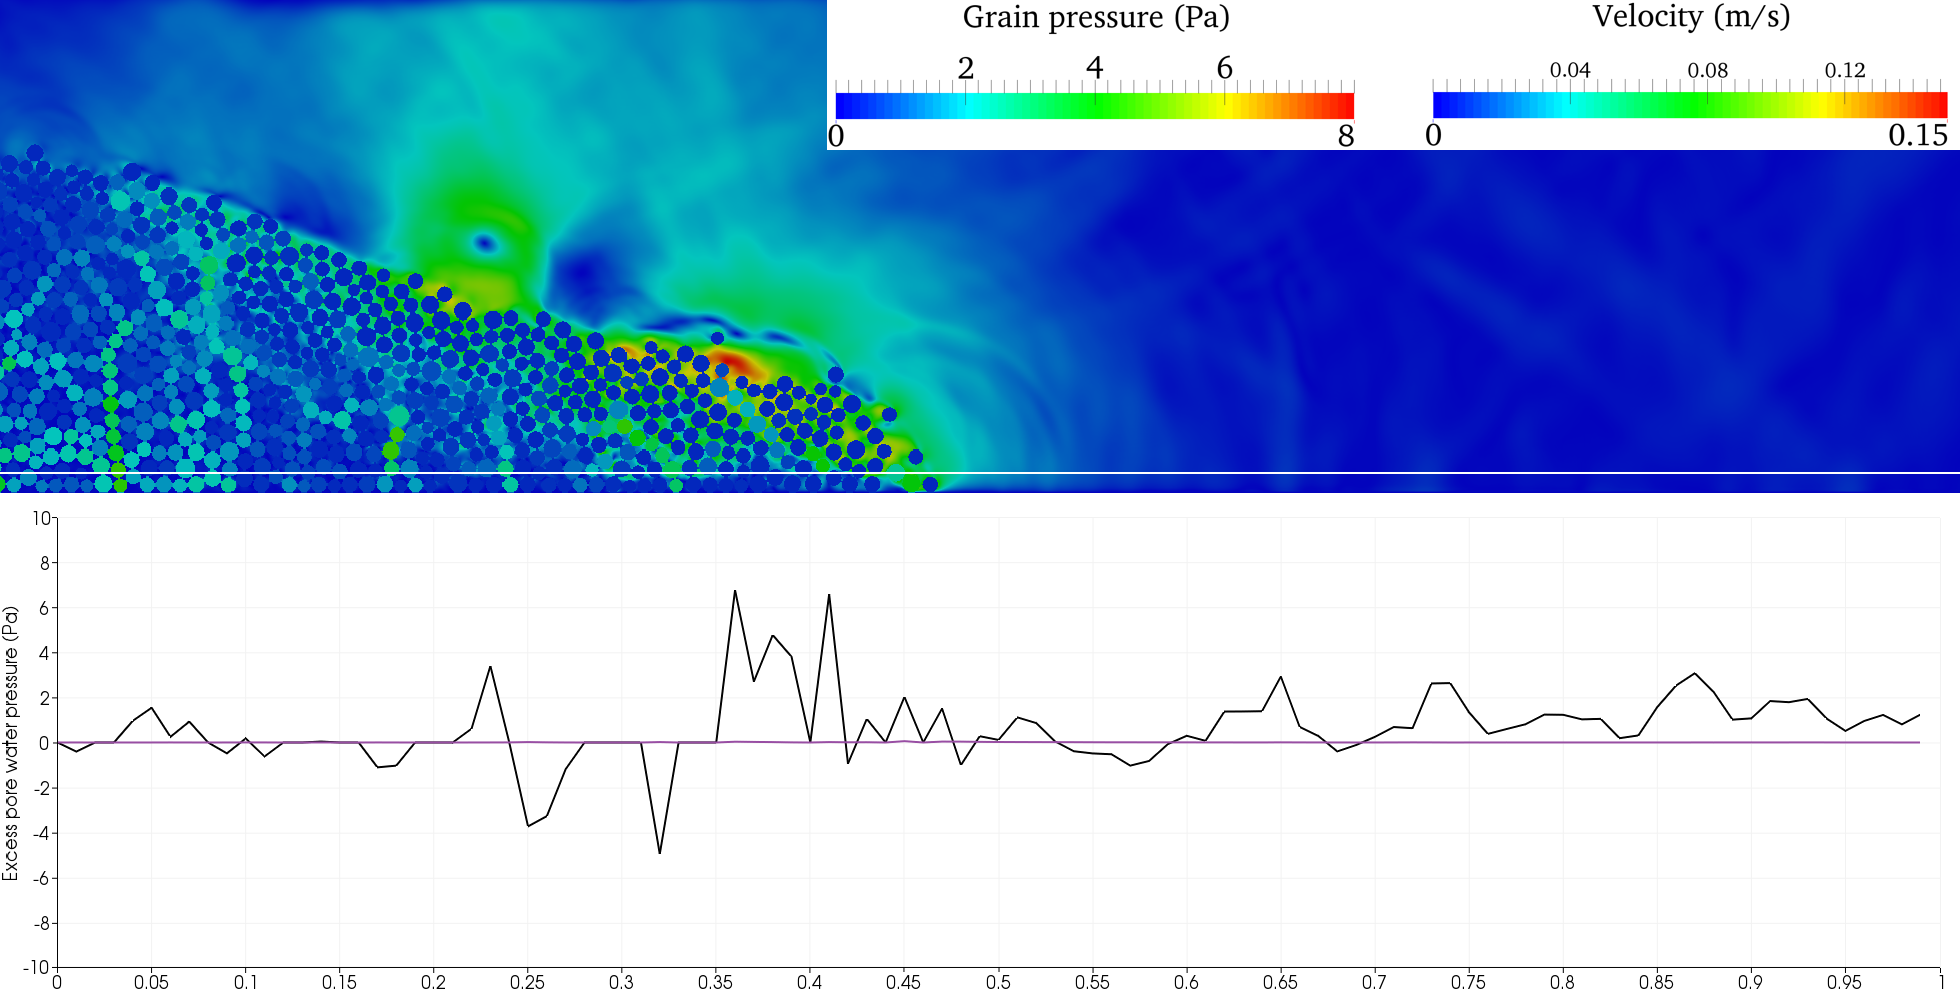
\includegraphics[width=\linewidth]{figs/a08/r07_PWP_flow_dense}
    \caption{High permeability (\textit{r} = 0.7 \textit{R}) - Pressure at the 
    bottom of the granular flow.}
    \label{fig:r07_PWP_flow_dense}
\end{subfigure}
\\
\begin{subfigure}[t]{0.975\linewidth}
	\centering
    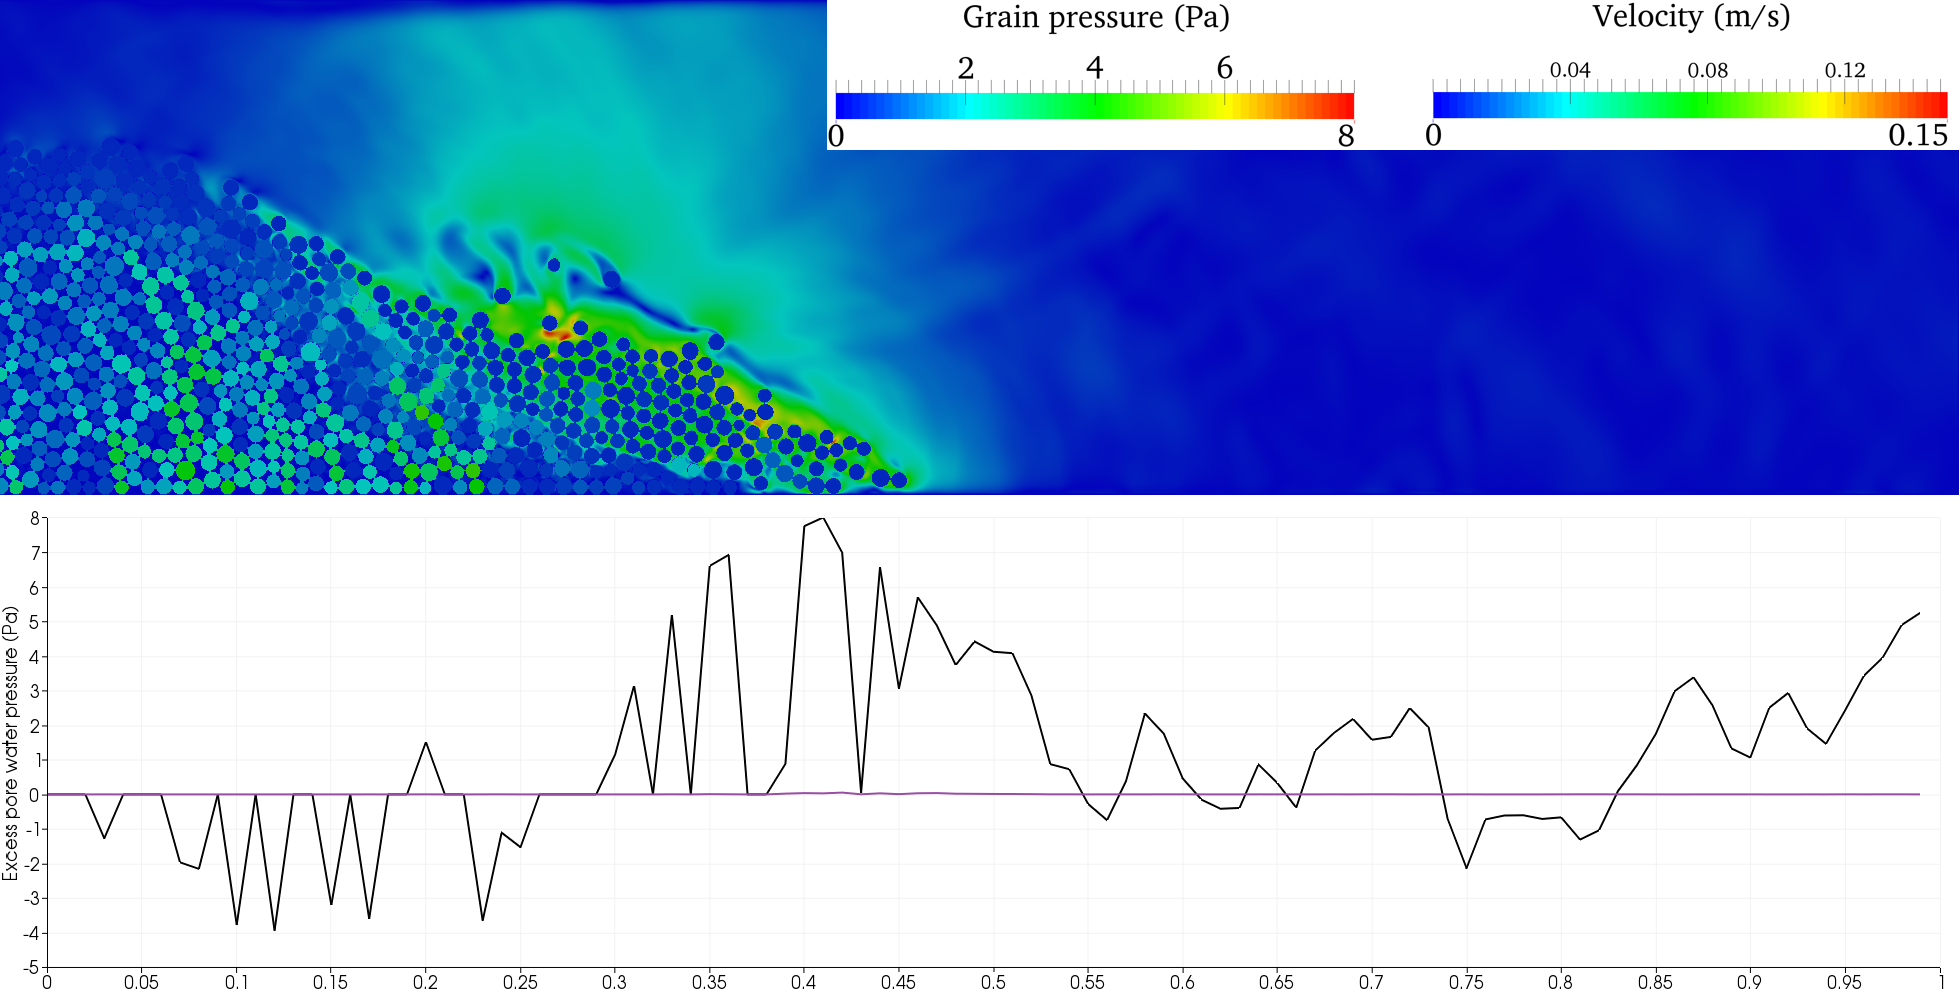
\includegraphics[width=\linewidth]{figs/a08/r095_PWP_flow_dense}
    \caption{Low permeability (\textit{r} = 0.95 \textit{R}) - Pressure at the 
        bottom of the granular flow.}
    \label{fig:r095_PWP_flow_dense}
\end{subfigure}
\caption{Effect of permeability on the excess pore water pressure distribution 
along the bottom plane for a granular column collapse in fluid (a = 0.8 \& 
dense packing) at $t = 2\tau_c$.}
\label{fig:PWP_flow_dense}
\end{figure}

\begin{figure}
\centering
\makebox[\linewidth][c]{
\begin{subfigure}[t]{0.95\linewidth}
	\centering
    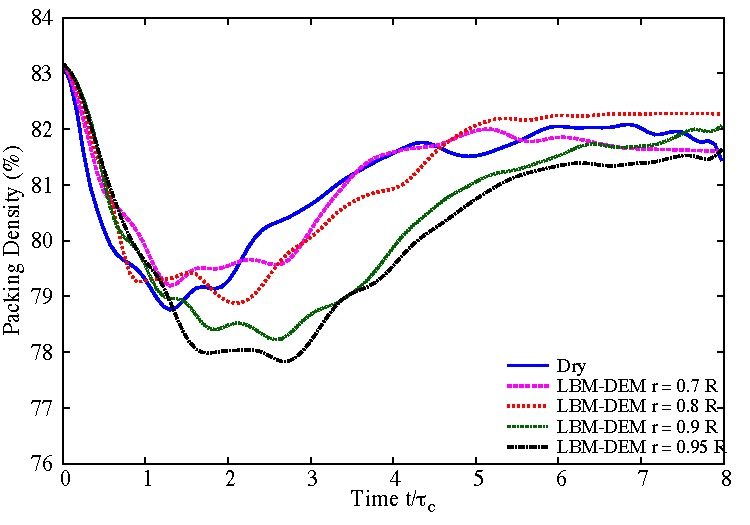
\includegraphics[width=0.8\linewidth]{figs/Packing_Density_a08_dense}
    \caption{Evolution of the packing density.}
    \label{fig:Packing_Density_a08_dense}
\end{subfigure}
}\\

\makebox[\linewidth][c]{
\begin{subfigure}[t]{0.95\linewidth}
	\centering
    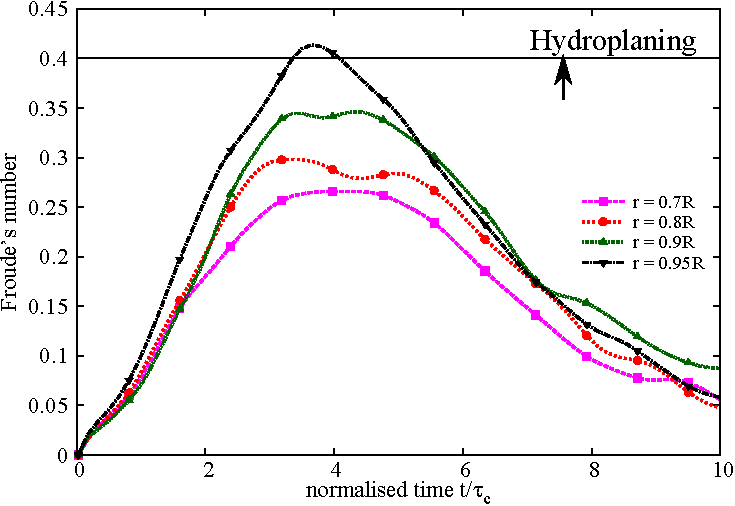
\includegraphics[width=0.8\linewidth]{figs/Fr_a08_dense}
    \caption{Evolution of the Froude's number.}
    \label{fig:Fr_a08_dense}
\end{subfigure}
}
    \caption{Effect of permeability on the evolution of packing density and 
    Froude's number for a granular column collapse in fluid (a = 0.8 \& dense 
    initial packing).}
    \label{fig:Packing_Density_Fr_a08_dense}
\end{figure}


\Cref{fig:Packing_Density_a08_dense} shows that the high permeability granular
column shows lower water entrainment (smaller decrease in packing denisty),
which indicates that for highly 
permeable flows the drag force acting on the soil grains predominates over the 
lubrication effect on the run-out behaviour.~\Cref{fig:Fr_a08_dense} shows the 
evolution of Froude's number with time for different permeability conditions. 
In dense granular columns, the Froude's number increases with decrease in 
permeability, however the Froude's number is below a critical value of 0.4 even 
for a low permeable column. Hence, no hydroplaning is observed. In both the low 
and high permeable granular flows, the granular material consolidates at the 
final stage of the flow (\cref{fig:Packing_Density_a08_dense}). This can be 
observed by the increase in the packing density at the final stage due to 
settlement of grains and expulsion of entrained water.

\subsection{Loose granular collapse}

The normalised run-out evolution with time for a loose initial packing (79\% 
packing fraction) with different hydrodynamic radii 0.7 \textit{R} to 0.95
\textit{R} are presented in~\cref{fig:Runout_a08_loose}. The 
run-out evolution a column of grains in suspension is compared with the dry and 
submerged granular columns to understand the influence of hydrodynamic forces 
on the flow kinematics. Similar to the dense granular column, the run-out 
distance increases with increase in the hydrodynamic radius (i.e., decrease in 
permeability). At low permeabilities (\textit{r} = 0.9 and 0.95 \textit{R}), 
the run-out distance is longer than the dry condition. This shows that the 
lubrication effect in low permeability conditions overcomes the influence of 
the drag force and the development of large negative pore-pressure resulting in 
a longer run-out distance. Although the suspended granular masses experience 
higher drag forces and turbulent effects, the run-out evolves almost at the 
same rate in comparison with granular columns with high permeability. This 
shows the effect of permeability on the dissipation rate of negative 
pore-pressure developed during the initial stage of collapse.

\begin{figure}
\centering
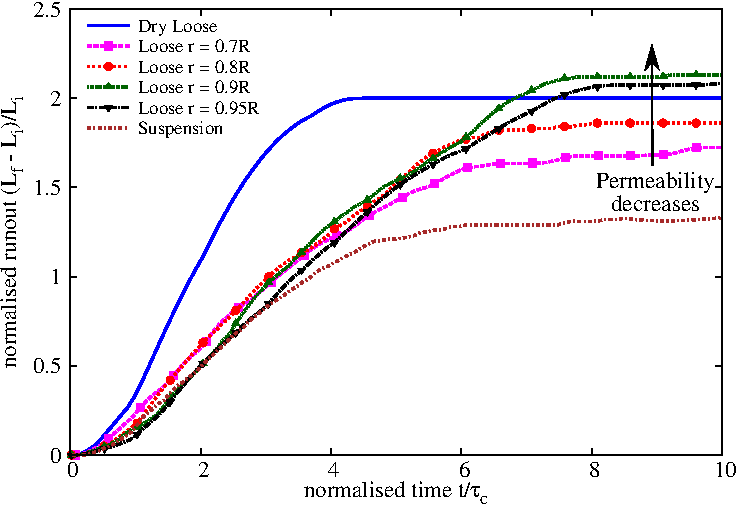
\includegraphics[width=0.9\linewidth]{figs/Runout_a08_loose.pdf}
\caption{Effect of permeability on the evolution of run-out for a column 
collapse in fluid (a = 0.8 \& loose packing).}
\label{fig:Runout_a08_loose}
\end{figure}

\Cref{fig:Loose_PWP_ini} shows the development of negative pore-pressure in low 
permeability (\textit{r} = 0.95 \textit{R}) and dissipation of negative 
pore-pressure in high permeability (\textit{r} = 0.7 \textit{R}) at the same 
time $ t = \tau_c$. This difference in the quantity and the rate of dissipation 
of negative pore-pressure results in a difference in the rate of flow 
evolution. A low permeability column requires a longer duration to 
evolve.~\Cref{fig:Loose_PWP_flow} shows the distribution of the excess 
pore-pressure along the bottom for low and high permeability conditions. As the 
flow progresses, the low permeability of the granular column causes 
hydroplaning to occur at the base of the column, which can be observed by high 
positive pore-pressure at the base of the flow front 
(\cref{fig:Loose_r095_PWP_flow}), resulting in a 
longer run-out distance.

\begin{figure}
\centering
\makebox[\linewidth][c]{
\begin{subfigure}[t]{0.975\linewidth}
	\centering
    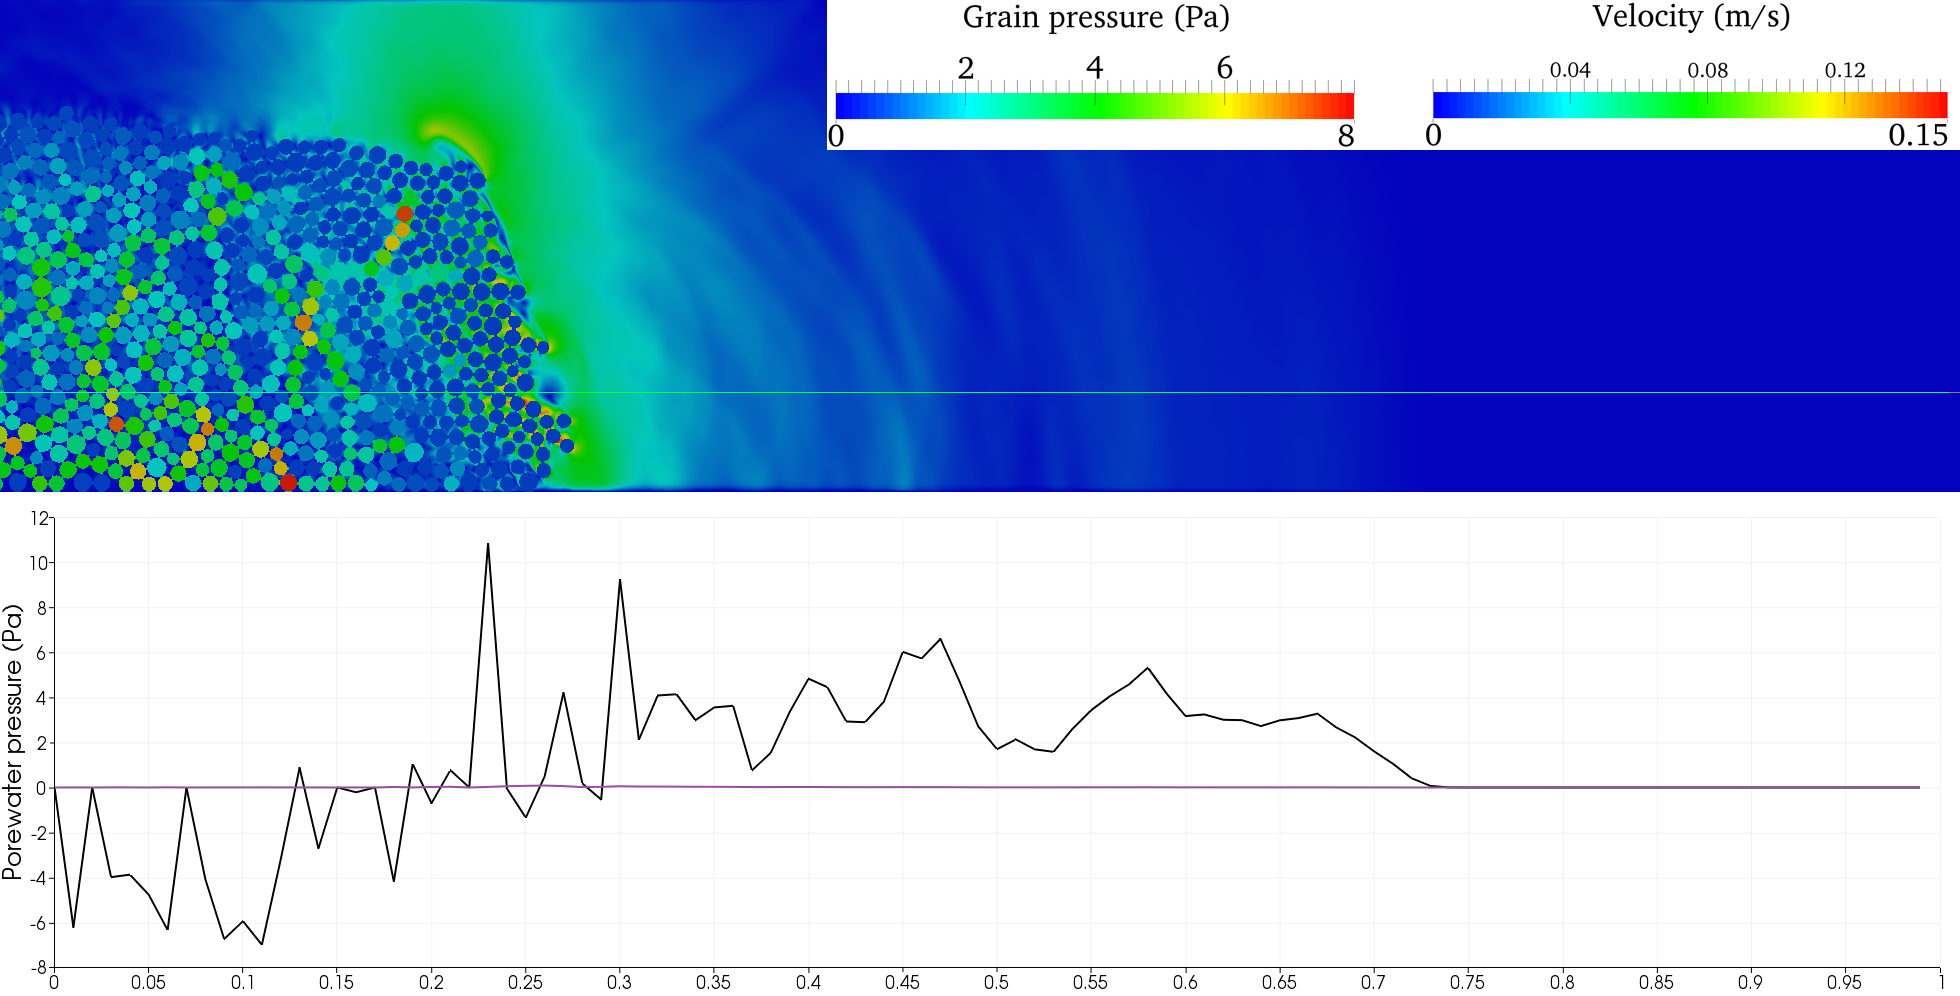
\includegraphics[width=\linewidth]{figs/a08/Loose_r07_PWP_ini}
    \caption{High permeability (\textit{r} = 0.7 \textit{R}) - Pressure at the 
        bottom of the granular flow.}
    \label{fig:Loose_r07_PWP_ini}
\end{subfigure}
}\\
\makebox[\linewidth][c]{
\begin{subfigure}[t]{0.975\linewidth}
	\centering
    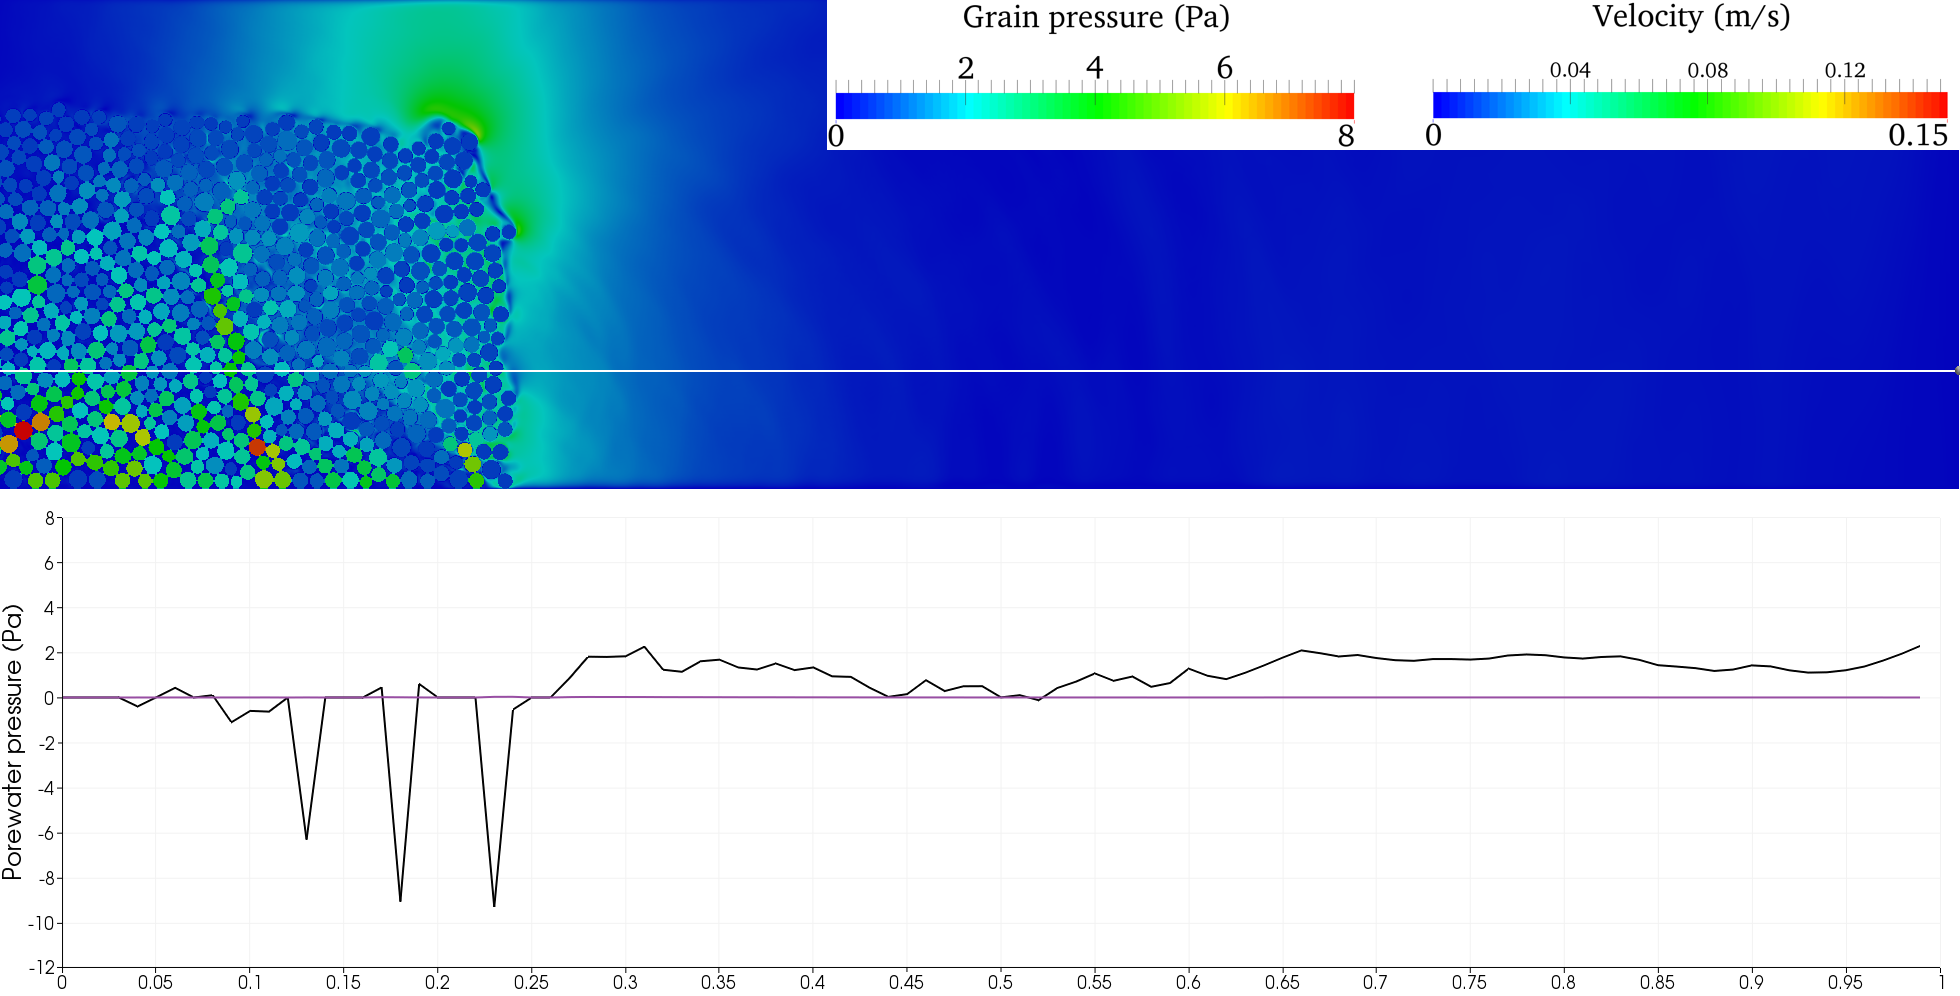
\includegraphics[width=\linewidth]{figs/a08/Loose_r095_PWP_ini}
    \caption{Low permeability (\textit{r} = 0.95 \textit{R}) - Pressure at the 
    bottom of the granular flow.}
    \label{fig:Loose_r095_PWP_ini}
\end{subfigure}
}
\caption{Effect of permeability on the excess pore water pressure distribution 
along the base of a granular column collapse in fluid (a = 0.8 \& loose 
packing) at $t = \tau_c$.}
\label{fig:Loose_PWP_ini}
\end{figure}

\begin{figure}
\centering
\makebox[\linewidth][c]{
\begin{subfigure}[t]{0.975\linewidth}
	\centering
    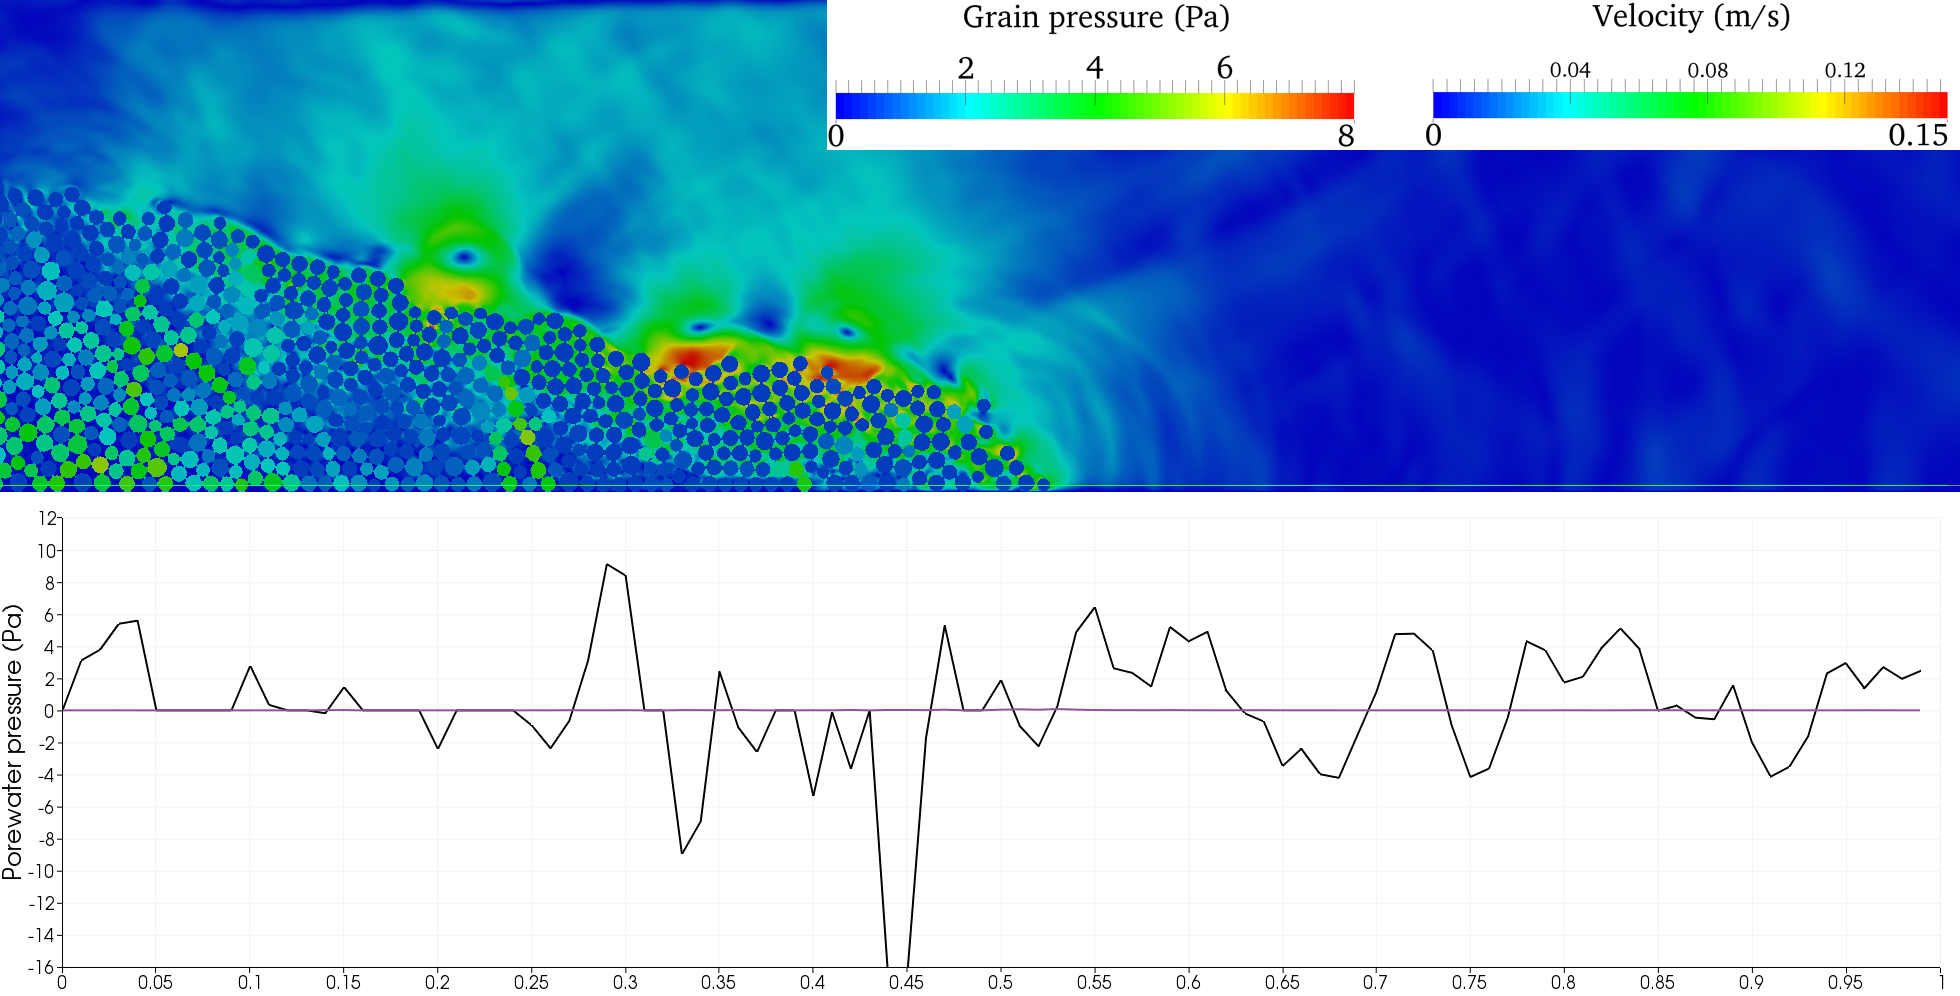
\includegraphics[width=\linewidth]{figs/a08/Loose_r07_PWP_flow}
    \caption{High permeability (\textit{r} = 0.7 \textit{R}) - Pressure at the 
        bottom of the granular flow.}
    \label{fig:Loose_r07_PWP_flow}
\end{subfigure}
}\\
\makebox[\linewidth][c]{
\begin{subfigure}[t]{0.975\linewidth}
	\centering
    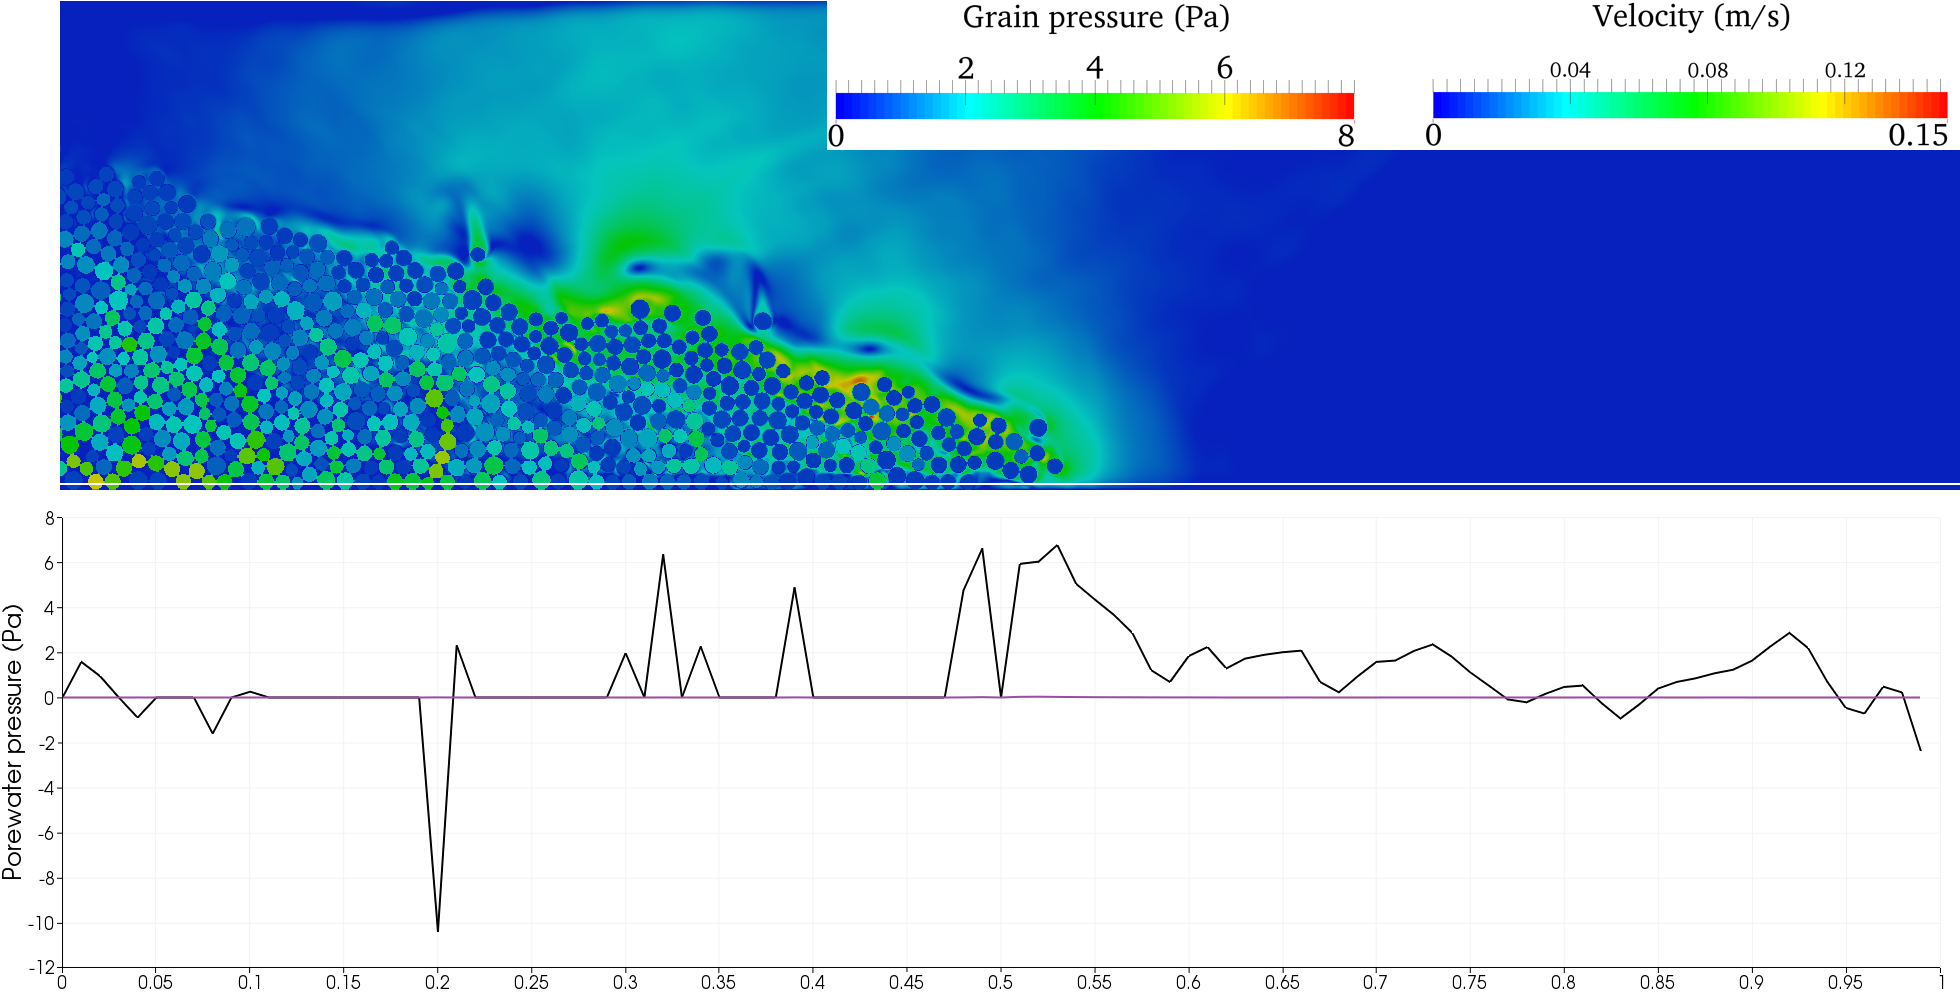
\includegraphics[width=\linewidth]{figs/a08/Loose_r095_PWP_flow}
    \caption{Low permeability (\textit{r} = 0.95 \textit{R}) - Pressure at the 
        bottom of the granular flow.}
    \label{fig:Loose_r095_PWP_flow}
\end{subfigure}
}
\caption{Effect of permeability on the excess pore water pressure distribution 
for a granular column collapse in fluid (a = 0.8 \& loose packing) at $t = 
2\tau_c$.}
\label{fig:Loose_PWP_flow}
\end{figure}

The initial potential energy mobilised is smaller than at \textit{r} = 0.9 
\textit{R}. Also with decreasing permeability, the time required to 
dissipate the negative pore-pressure increases. This results in a shorter 
run-out distance in the case of \textit{r} = 0.95 \textit{R} to that of 
\textit{r} = 0.9 \textit{R}. As the quantity of material destabilised is small, 
the flow is thinner and thus has a high Froude's number 
(0.59).~\Cref{fig:KExy_a08_loose} shows that the peak horizontal kinetic 
velocity observed in the case of \textit{r} = 0.9 \textit{R} is higher than 
\textit{r} = 0.95 \textit{R}. A Froude's number of 0.59 for \textit{r} = 0.9 
\textit{R} is observed in contrast to 0.46 for \textit{r} = 0.95 \textit{R}. 
Both values of hydrodynamic radii result in a Froude's number that indicate the 
occurrence of hydroplaning. However, the difference in the amount of material 
destabilised for \textit{r} = 0.95 \textit{R} and the decreased effect of 
hydroplaning results in a shorter run-out distance for \textit{r} = 0.95 
\textit{R} in comparison to \textit{r} = 0.9 \textit{R}.


\Cref{fig:Packing_Density_a08_loose} shows the evolution of packing 
fraction with time for different values of permeability. As the column 
collapses, water is entrained at the flow front. This can 
observed by the decrease in the packing fraction during $t = \tau_c$ and $t = 
3\tau_c$. As the flow progresses, the entrained water is expelled and the soil 
grains consolidate to reach a critical packing density at the end of the flow. 
The permeability (i.e., hydrodynamic radius) plays a crucial role in the rate 
of dissipation of the entrained water. As the permeability decreases, the water 
entrained at the flow front takes longer time to be dissipated resulting in 
lubrication of the flow at low permeabilities.~\Cref{fig:Fr_a08_loose} shows 
that the low permeable columns exhibit higher Froude's numbers, greater than 
0.4, that indicates occurrence of hydroplaning. This lubrication effect results 
in an increase in the run-out distance for columns with low permeabilities.


\begin{figure}
    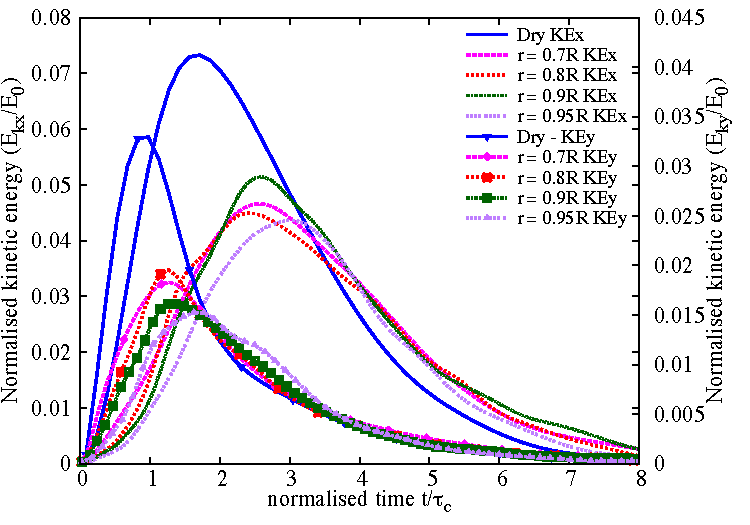
\includegraphics[width=\linewidth]{figs/KExy_a08_loose}
    \caption{Effect of permeability on the evolution of kinetic energies with time 
for a granular column collapse in fluid (a = 0.8 \& loose packing).}
    \label{fig:KExy_a08_loose}
\end{figure}

\begin{figure}
\centering
\makebox[\linewidth][c]{
\begin{subfigure}[t]{0.95\linewidth}
	\centering
    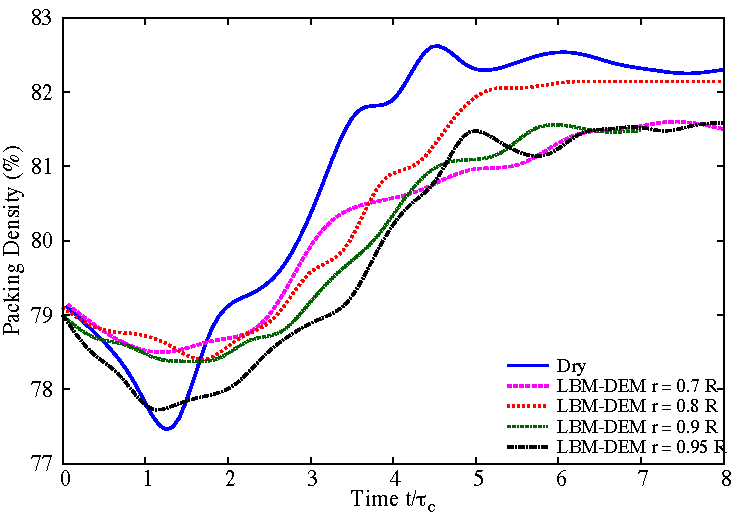
\includegraphics[width=0.8\linewidth]{figs/Packing_Density_a08_loose}
    \caption{Evolution of packing density.}
    \label{fig:Packing_Density_a08_loose}
\end{subfigure}
}\\
\makebox[\linewidth][c]{
\begin{subfigure}[t]{0.95\linewidth}
	\centering
    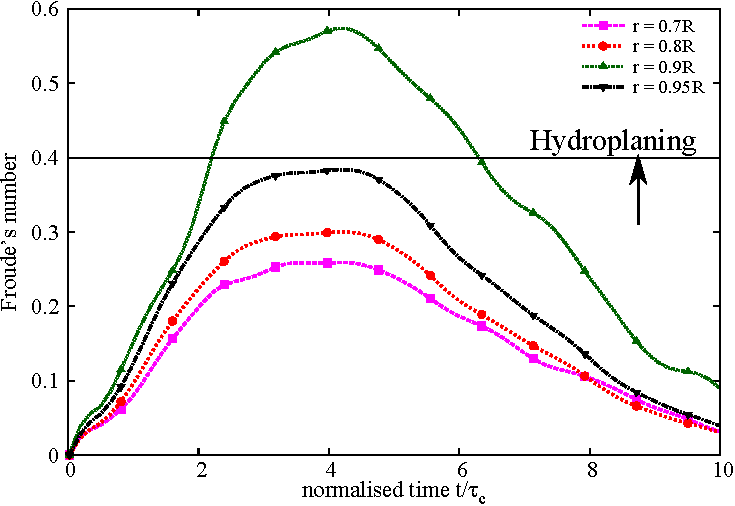
\includegraphics[width=0.8\linewidth]{figs/Fr_a08_loose}
    \caption{Evolution of Froude's number.}
    \label{fig:Fr_a08_loose}
\end{subfigure}
}
    \caption{Effect of permeability on the evolution of packing density and 
    Froude's number for a granular column collapse in fluid (a = 0.8 \& loose 
    initial packing).}
    \label{fig:Packing_Density_Fr_a08_loose}
\end{figure}

\Cref{fig:Dense_Loose_PT} shows the grain trajectories of a dense and a loose 
initial packing for a hydrodynamic radius (\textit{r} = 0.95 \textit{R}). It 
can be observed that 
the dense initial packing results in a lot of turbulent behaviour at the flow 
surface in contrast to the more uniform flow behaviour in the loose condition. 
The thickness of the deposit in both dense and loose condition is almost the 
same, however the density of the flow results in a Froude's number of 0.59 and
0.429 for loose and dense conditions, respectively. The low initial density 
results in more hydroplaning in the loose condition.
Comparing the evolution packing densities in dense and loose conditions
(\cref{fig:Packing_Density_a08_dense,fig:Packing_Density_a08_loose}) 
reveal almost the same packing density when the flow is fully mobilised. Hence, 
it is the density of the flowing granular mass that controls the influence of 
hydroplaning for a given hydrodynamic radius and initial aspect ratio. A 
loosely packed granular column with low permeability entrains 
more water at the flow front, resulting in a hydroplaning effect that overcomes 
the influence of viscous drag forces and thereby yields a higher run-out 
distance than the dry condition.


\begin{figure}[htbp]
\centering
\makebox[\linewidth][c]{
\begin{subfigure}[t]{0.8\linewidth}
	\centering
    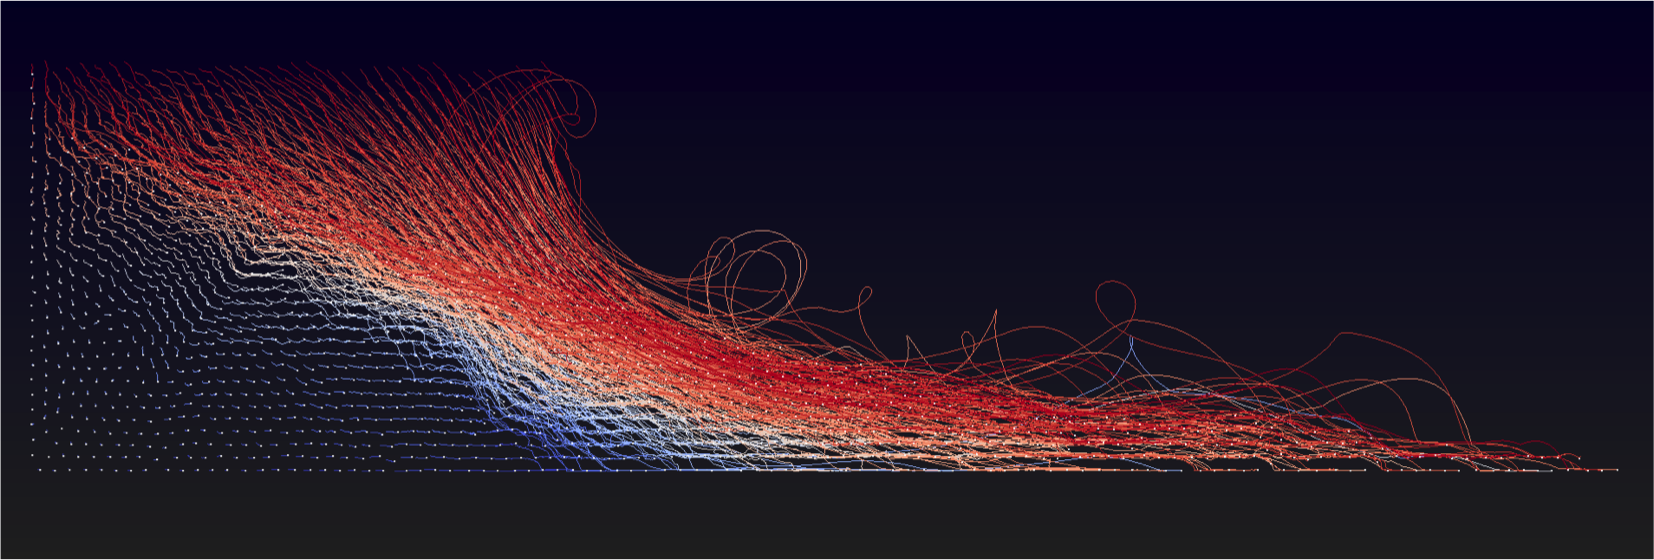
\includegraphics[width=\linewidth]{figs/a08/PT_Dense_R095}
    \caption{Dense initial packing (83\%)}
    \label{fig:PT_Dense_R095}
\end{subfigure}
}\\
\makebox[\linewidth][c]{
\begin{subfigure}[t]{0.8\linewidth}
	\centering
    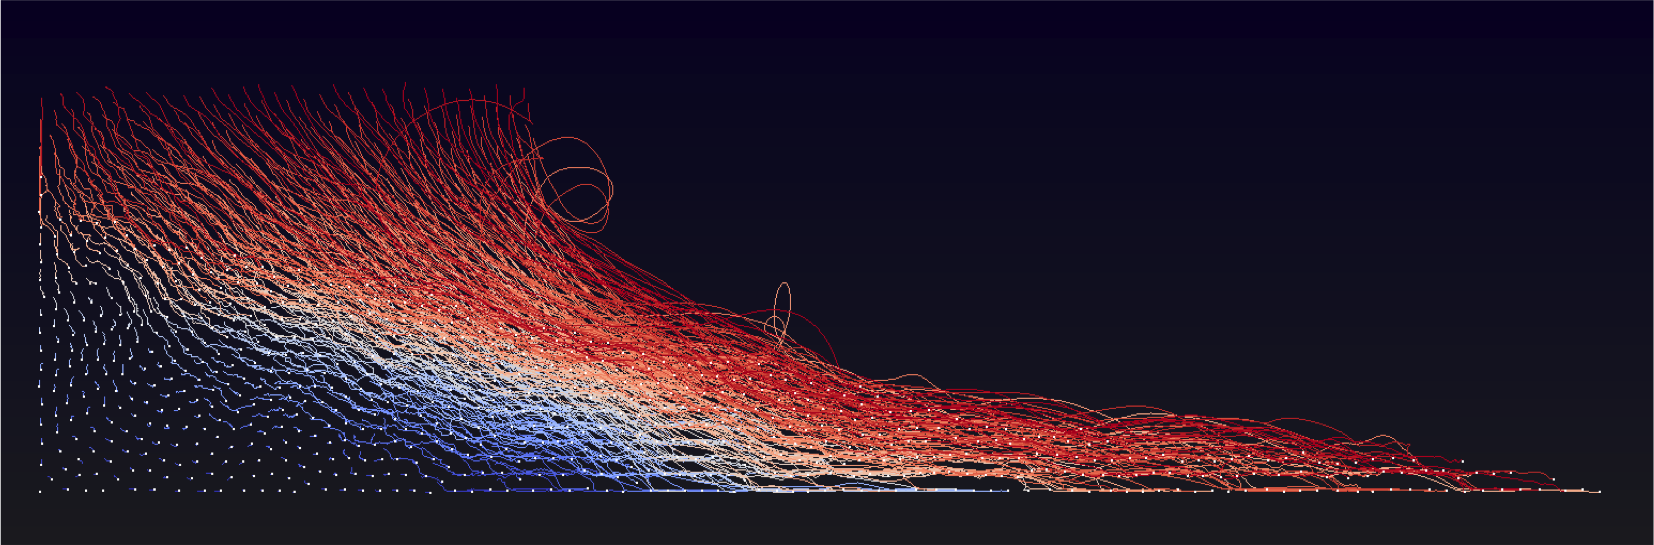
\includegraphics[width=\linewidth]{figs/a08/PT_Loose_R095}
    \caption{Loose initial packing (79\%)}
    \label{fig:PT_Loose_R095}
\end{subfigure}
}
\caption[Effect of initial density on the deposit morphology
for a granular column collapse in fluid (a = 0.8).]{Effect of initial density 
on the deposit morphology
for a granular column collapse in fluid (a = 0.8). Dense vs. loose initial 
packing fraction (\textit{r} = 0.95 \textit{R}). Darker means dense packing, 
white indicates loose packing density.}
\label{fig:Dense_Loose_PT}
\end{figure}

\section{Summary}

Two-dimensional LB-DEM simulations were performed to understand the behaviour of
submarine granular flows. Unlike dry granular collapse, the run-out behaviour in
fluid is dictated by the initial volume fraction. 
\shortciteN{Rondon2011} experimentally observed that the collapse of a granular
column in a viscous fluid is mainly controlled by the initial volume fraction and
not by the aspect ratio of the column. The role of the initial volume fraction 
observed explains the pore pressure feedback mechanism proposed 
by~\shortciteN{Schaeffer2008} in the context of landslides. The dense column
needs to dilate in order to flow. When it starts to fall, liquid is then sucked
into the column, which is then stabilised by the additional viscous drag. By
opposition the loose column when it starts flowing expands and ejects liquid,
leading to a partial fluidisation of the material.

\bibliographystyle{chicaco}
\bibliography{references}

\end{document}
